\documentclass[11pt]{article}
%Gummi|061|=)
\title{\textbf{The flume problem in the centre plane.}}
\author{Nicolas}
\date{}
\usepackage{graphicx}
\usepackage{amsmath}
\usepackage[left=2cm,right=2cm,top=2cm,bottom=2cm]{geometry}
\newcommand{\p}[2]{\ensuremath{\frac{\partial {#1}}{\partial {#2}}}}
\newcommand{\tot}[2]{\ensuremath{\frac{d {#1}}{d {#2}}}}

\newcommand{\hphi}{\ensuremath{\hat{\phi}}}
\newcommand{\z}{\ensuremath{\zeta}}
\newcommand{\x}{\ensuremath{\xi}}
\newcommand{\zperp}{\ensuremath{\zeta^\perp}}
\newcommand{\lam}{\ensuremath{\lambda}}

\begin{document}

\maketitle

\section{Goal and idea}
We want to solve the segregation equation
\begin{equation} \label{eq:conservative_form}
	\p{\phi}{t} + \p{u\phi}{x} + \p{v\phi}{y} + \p{w\phi}{z} - \p{\phi(1-\phi)}{z} = 0
\end{equation}

We are looking for a steady-state solution in the frame travelling at the (constant) speed of the front $u_F$. So by making the change of variable $ x \leftarrow x - u_F t$ we are left with

\begin{equation}
	\p{u\phi}{x} + \p{v\phi}{y} + \p{w\phi}{z} - \p{\phi(1-\phi)}{z} = 0
\end{equation}
We can make use of incompressibility, to take the velocity components out of the partial derivatives:
\begin{equation}
	u\p{\phi}{x} + v\p{\phi}{y} + w\p{\phi}{z} - \p{\phi(1-\phi)}{z} = 0
\end{equation}
and since $v = 0$ in the centre plane, we have
\begin{equation} \label{eq:segreg}
	u\p{\phi}{x} + w\p{\phi}{z} - \p{\phi(1-\phi)}{z} = 0
\end{equation}
Our goal is to find a solution of this equation, given the physical setup of the flume problem.

\subsection{Method of the characteristics}
We can rewrite \cite{eq:segreg} as 
\begin{equation} \label{eq:carac_form}
		u\p{\phi}{x} + w\p{\phi}{z} - (1 - 2\phi)\p{\phi}{z} = 0
\end{equation}
The steady-state solution is a function of 2 variables: $ \phi = \phi(x, z)$. So the solution can be seen as the surface $ \phi - \phi(x,z) = 0$ of the 3D space $(x, z, \phi)$. 
Characteristics are curves $\phi = \hphi(x(s),z(s))$ lying on this surface, and verifying
\begin{equation}
	\frac{d \hphi}{d s} = 0
\end{equation}
Using chain rule we have 
\begin{equation}
	\p{x}{s} \p{\hphi}{x} + 
	\p{z}{s}\p{\hphi}{z} = 0
\end{equation} 
and since $\hphi$ is lying on the solution surface,
\begin{flalign}
\p{x}{s} = u \\
\p{z}{s} = w - (1- 2 \hphi)
\end{flalign}
Rather than using a parameter $s$, we can directly express $z$ as a function of $x$, and since 
\begin{equation}
	\p{z}{s} = \p{x}{s} \frac{d z}{d x} 
\end{equation} 
we have
\begin{equation} \label{eq:charac}
	u \frac{d z}{d x} = w - (1- 2 \hphi)
\end{equation}

This characteristic equation is exactly the one we have for a 2D problem\footnote{For example it is equation (2.6) in Thornton and Gray 2008, Breaking size segregation waves and particle recirculation in granular avalanches.}.
It has proved useful for these 2D problems to remap the $z$ axis so that characteristic curves given by \cite{eq:charac} become straight lines.

In the next section I will sum up how we tried to apply this method to ou 3D problem.

\section{What we tried}

\subsection{Changing the coordinates}

In the 2D case, the idea was to remap the $z$ axis: 
\begin{equation}
	z \leftarrow \psi(x,z)
\end{equation}
Where $\psi$ is the stream function defined by 
\begin{equation}
	\begin{pmatrix}
	\p{\psi}{x}\\
	\p{\psi}{z} 
\end{pmatrix}
=
	\begin{pmatrix}
	-w\\
	u 
\end{pmatrix}
\end{equation}

Using the symmetry of second derivatives we see that the definition of $\psi$ implies
\begin{equation}
	\p{u}{x} + \p{w}{z} = 0
\end{equation}
which is the incompressibility condition for a 2D flow. Of course in 3D the incompressibility condition is
\begin{equation}
	\p{u}{x} + \p{v}{y} + \p{w}{z} = 0
\end{equation}
so we cannot define a stream function.
We need to use another function to remap the $z$ axis.

We notice that for a 2D stationary flow, the lines $\psi(x,z) = 0$ are the particle paths \footnote{Note that for a granular polydisperse flow, what we call "particle paths" are not the paths followed by actual particles. It is rather  the paths of hypothetical particles having their velocity equal to the bulk velocity.}.
So in the 3D case, rather than remapping the $z$ axis with a stream function, which is impossible, we will just say that our new $z$ coordinate is a -for now- unknown function $\z(x,z)$ which is constant along particle paths.

This property imply that
\begin{equation}
	\begin{pmatrix}
	\p{\z}{x}\\
	\p{\z}{z} 
\end{pmatrix}
\propto
	\begin{pmatrix}
	-w\\
	u 
\end{pmatrix}
\end{equation}
Let us call $\lam(x,z)$ the coefficient of proportionality. Of course if $\lam(x,z) = 1$ we have again
\begin{equation}
	\p{u}{x} + \p{w}{z} = 0
\end{equation}
so let us assume to begin with that $\lam$ is a function of $\zeta$ only : $\lam(x,z) = \hat{\lam}(\z)$

Expressing the velocity components in terms of derivatives of $\z$ in the 3D incompressibility equation yields
\begin{equation} \label{eq:lambda}
	- \underbrace{  \left( u \p{}{x} + w\p{}{z}\right) }_{\equiv D^\perp}  \log \lam(x,z) + \p{v}{y} = 0
\end{equation}
The operator $D^\perp$ appearing in the formula above plays a particular role.
Indeed if we call $\zperp$ the coordinate locally orthogonal to $\zeta$ we can easily see that
\begin{equation}
	D^\perp = u \p{}{x} + w\p{}{z} \propto \p{}{\zperp}
\end{equation}
so, if $\lam(x,z) = \hat{\lam}(\z)$ we have $D^\perp \hat \lam(\z) = 0$ and thus again
\begin{equation}
	\p{u}{x} + \p{w}{z} = 0
\end{equation}

Since making $\lam$ dependant or not on $\z$ does not have any impact on  \cite{eq:lambda} I am going to assume for now on that $\lam$ is not a function of $\z$. In the system of coordinates $(x, \z)$ I am going to define $\lam$ as a function of $x$ only : $\lam = \lam(x)$.
In this system of coordinates, $D^\perp = u \p{}{x}$ and thus
\begin{equation}
	-u \tot{}{x} \log \lam + \p{v}{y} = 0
\end{equation}

Integrating this first order ODE will give us $\lam(x)$ up to an arbitrary integration constant. Knowing $\lam(x)$, we can in turn know $\z(x,z)$, again up to an integration constant, using
\begin{equation}
	\begin{pmatrix}
	\p{\z}{x}\\
	\p{\z}{z} 
\end{pmatrix}
=
\lam(x)
	\begin{pmatrix}
	-w\\
	u 
\end{pmatrix}
\end{equation}
If we do that, we will have completely defined our change of coordinate $z \leftarrow \z$ and we will know it explicitly.
But is it useful to do this change of coordinates? Does it make it easier to find the structure of the steady-state solution as in the 2D case? We will see that it is indeed the case in the next section.

\subsection{Applying the change of coordinates to the segregation equation}

After the change of coordinate, the segregation equation \cite{eq:segreg} becomes
\begin{equation}
	\p{\phi}{x} - \lam(x) \p{}{\z} \phi (1 - \phi) = 0
\end{equation}
This equation is exactly the one we have in the 2D case, after doing the change of coordinate $z \leftarrow \z(x,z)=\psi(x,z)$, except that in that case $\lam(x) = 1$.

Let $\z = Z(x)$ be a characteristic curve. And let us call $\Phi$ the (constant) value of  $\phi(x,\z)$ along the characteristic curve. We have
\begin{equation}
	\tot{Z}{x} = - \lam(x) ( 1 - 2 \Phi)
\end{equation}
Because $\lam$ depends on $x$ characteristics are not straight lines, contrary to what happens in the 2D case. 
At that point, Parmesh suggested that we remap also the $x$ axis : $x \leftarrow \x(x)$. 
In this new system of coordinates, characteristics will be straight lines iff
\begin{equation}
	\tot{\x}{x} = \lam(x)
\end{equation}
and the segregation equation becomes
\begin{equation}
	\p{\phi}{\x} - \p{}{\z} \phi (1 - \phi) = 0
\end{equation}

In this new coordinates system the jump condition is of course simply the same as in 2D :
\begin{equation}
	\tot{\z}{\x} = \phi^+ + \phi^-  - 1
\end{equation}

The equation is the same as in 2D case, but we expect the solution to be different. Namely, to exhibit a "spiral" rather than a "lens" structure. 
Why is this spiral appearing? Parmesh's feeling when I talked with him about it was that since the horizontal and vertical coordinates $\x$ and $\z$ can \textit{both} take the same value for different values of $x$ and $z$\footnote{in other words the inverse mapping $x = x(\x, \z)$ and $z = z(\x,\z)$ is multivalued}, the spatial domain in the remapped coordinates is a mosaic of smaller domains inside which $\x$ and $\z$ do not take the same value for different values of $x$ and $z$, each small domain forming a part of the spiral.
I do not have a clear intuition of how the small domains are arranged. I think it is best to try to do the actual computation of the remapped coordinates, with the prescribed velocity field used in the flume paper. This is the object of the next section.

\subsection{Application of the method to a prescribed velocity field}

First, we can try to compute $\lam(x,z)$\footnote{In the coordinates system $(x,\z)$ \lam is only a function of $x$, but int the coordinates system $(x,z)$ it is also a function of $z$} using 
\begin{equation}
	-D^\perp \log \lam + \p{v}{y} = 0
\end{equation}
Then, we can deduce $\z(x,z)$, and finally $\x(x)$ from $\z(x,z)$.
I tried to do this with different velocity fields.

This velocity field is rather complicated, so I didn't expected to be able to get an analytical expression for \lam, but I tried anyway.
From the known velocity profile we can compute $\partial v / \partial y$:
\begin{equation}
	\p{v}{y}\bigg|_{y=0} = 
\frac{(2 n+1) U }{H (2 m+1) W (2 m+2 n+1)}
\text{csch}\left(\frac{x}{W}\right) \text{sech}\left(\frac{x}{W}\right) \left(2 (\alpha -1) z-\alpha  H \sqrt{-\tanh \left(\frac{x}{W}\right)}\right)
\end{equation}

The expressions for $u$ and $w$ are
\begin{align}
	u(x, z) = 
	\left(\alpha -\frac{2 (\alpha -1) z}{H \sqrt{-\tanh \left(\frac{x}{W}\right)}}\right) \left(\frac{(2 n+1) U \sqrt{-\tanh \left(\frac{x}{W}\right)}}{(2 m+1) (2 m+2 n+1)}+\text{uF}\right)-\text{uF} \\
	w(x,z) = \frac{-z}{2 H W}
	\text{csch}\left(\frac{x}{W}\right) \text{sech}\left(\frac{x}{W}\right) \left(\frac{(2 n+1) U \left(2 (\alpha -1) z-\alpha  H \sqrt{-\tanh \left(\frac{x}{W}\right)}\right)}{(2 m+1) (2 m+2 n+1)}+\frac{(\alpha -1) \text{uF} z}{\sqrt{-\tanh \left(\frac{x}{W}\right)}}\right)
\end{align}

It does not seem to be possible to solve the PDE to obtain $\lam$ directly (at least, I have not succeeded!). I have 3 ideas to work around this obstacle:

\begin{figure}[htp]
\centering
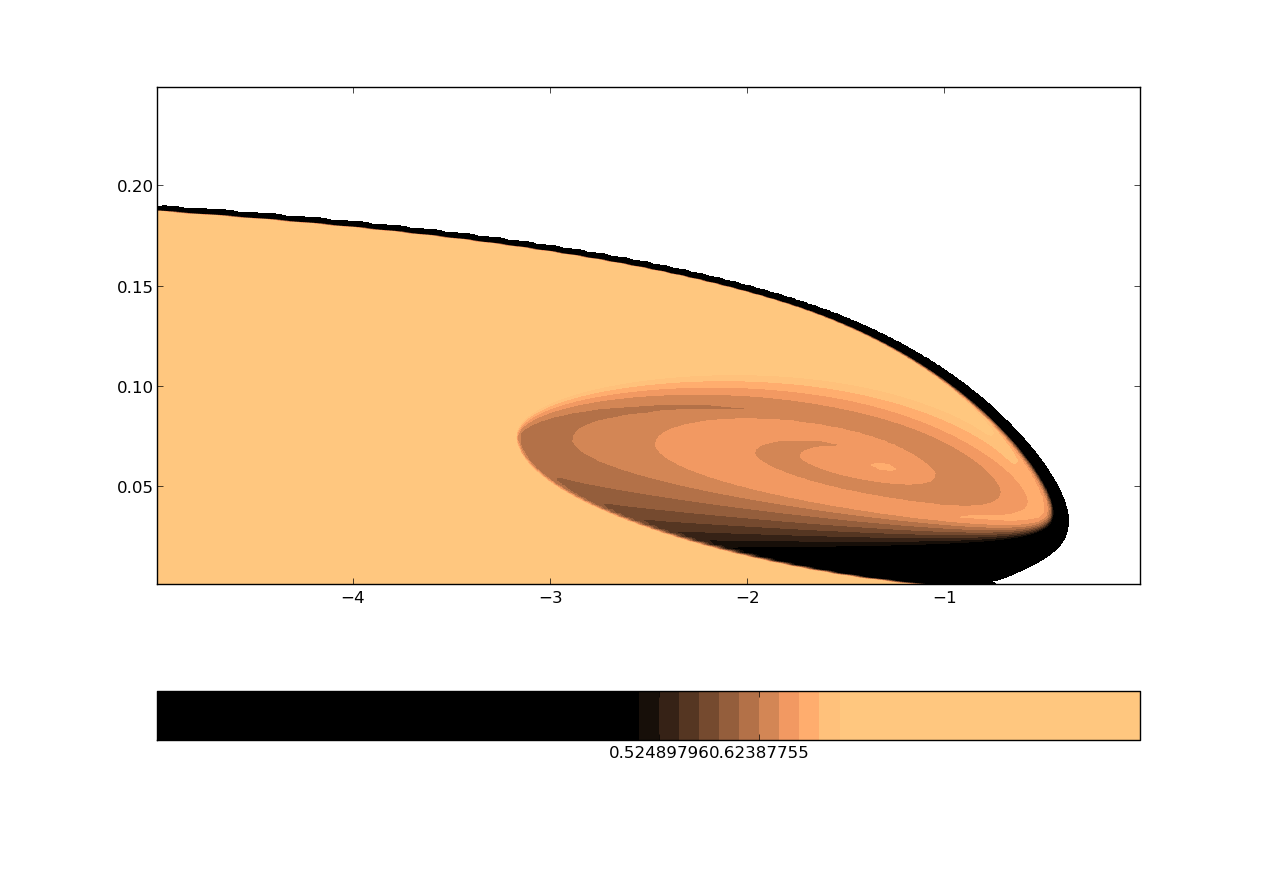
\includegraphics[scale=0.4]{rational_profile_spiral.png}
\caption{Numerical concentration in small particles for a velocity field constructed using a rational fraction of $x$ as the flow height}
\label{fig:2}
\end{figure}

\begin{itemize}
\item do a change of coordinates to simplify the equation on \lam. In particular any system of coordinates $(\hat z^\perp, \hat z)$ where $\hat z$ is constant along particle paths, and $\hat z^\perp$ orthogonal to $\hat z$ will transform the PDE into an ODE
\begin{equation}
	-\tot{}{\hat z^\perp} \log \lam(\hat z^\perp) + \p{v}{y} = 0
\end{equation}
but this implies finding the particle paths first, ie solving the ODE
\begin{equation}
	\tot{z}{x} = \frac{w}{u}
\end{equation}
which seems equally difficult.
\item find a simpler velocity field. I think what makes the equations hard to solve is the fact that the flow height is the coexistence of hyperbolic functions of $x$ and linear functions of $z$.
By replacing the hyperbolic height profile $h(x) = W \sqrt{ \text{tanh}(-x/H)}$ by a linear one $h(x) = - x/ (W - x) $ one can end up with differential equations only involving linear functions of $x$ and $z$, while preserving the spiral structure of the solution (see fig \cite{fig:2}).
This new profile indeed simplifies the expressions for velocity components a great deal, but I think it is still not possible to find the change a variable.
\item instead of prescribing the velocity field and try to find the change of variables, or the particle paths, prescribe the particle paths, and deduce the velocity field from that. It is what I will talk about in the next section.
\end{itemize} 

\subsection{Prescribing the particle paths}
We can deduce the particle paths (pp for short) from the velocity field using the kinematic equations for a particle in the flow:
\[
\begin{pmatrix}
	\frac{dx}{dt} \\
	\frac{dz}{dt} \\
\end{pmatrix}
=
\begin{pmatrix}
	u \\
	w \\
\end{pmatrix}
\]

Our problem is steady, so we can get rid of the time $t$ and express directly $z$ as a function of $x$ 
\[
\frac{dz}{dx}(x) = \frac{w(x, z)}{u(x, z)}
\]
This ODE may seem "easy" to solve, but I can't figure it out, even in the simple case $h(x) = h(x) = - x/ (W - x)$. In this case, the expressions for $u$ and $w$ are:
\[
 u =
 \left(
 \alpha 
 +\frac{2 (\alpha -1) z (W-x)}{H x}
 \right) 
 \left(
 u_F
 -\frac{(2 n+1) U x}{(2 m+1) (2 m+2 n+1) (W-x)}
 \right)-u_F
\]

\[
 w = 
 \frac{z \left(\frac{(2 n+1) U (x (\alpha  H-2 (\alpha -1) z)+2 (\alpha -1) W z)}{(2 m+1) (2 m+2 n+1)}-\frac{(\alpha -1) uF z (W-x)^2}{x}\right)}{H^2}
 \]
 
 
\section{Particle paths}

The idea is to deduce the velocity field from the prescribed pp, instead of doing the contrary.
Our first job is then to build a realistic set of pp. 
In other words we would like to find a set of $z_a(x)$ where $a$ is parameter classifying the pp.
Given the shape of the wanted particle paths, it seems to be easier to construct $x_a(z)$ rather than $z_a(x)$.
First we will define the parameter $a$. $a$ could be the height of the pp infinitely away form the head of the flow: $a = \text{lim}_{x \rightarrow -\infty} z(x) \doteq z_\infty$. We could also decide that $a$ will be the $x$ coordinate of the pp at which it "goes back" (\textit{ie} at the point where $dz/dx = - \infty$). 
Let's call this point $x_0$.

I have a good feeling about this function:
\[
z(x; x_0, z_\infty, z_0) = z_0 + (z_\infty - z_0) \sqrt {\text{tanh} (-x + x_0)}
\]

Indeed we have 
\[
\begin{matrix}
	\lim_{x \rightarrow -\infty} z = z_\infty \\
	z(x_0) = z_0 \\
\end{matrix}
\]
as expected. For now $z$ is a function as 3 parameters, but only one, $a$, is needed.
Let's for example express $z_\infty$ and $z_0$ as functions of $a = x_0$. I choose
\[
\begin{matrix}
   z_\infty(x_0) = \text{tanh}(-1/x_0) \text{ if } z > z_0 \\
   z_\infty(x_0) = 1 - \text{tanh}(-1/x_0) \text{ if } z < z_0 \\
   z_0(x_0) = \frac{1}{2} \text{tanh}\left(\frac{-x_0}{x_0+1/\text{arctan}(1/2)}\right) 
\end{matrix}
\]

This gives us the following pp:

\begin{figure}[htp]
\centering
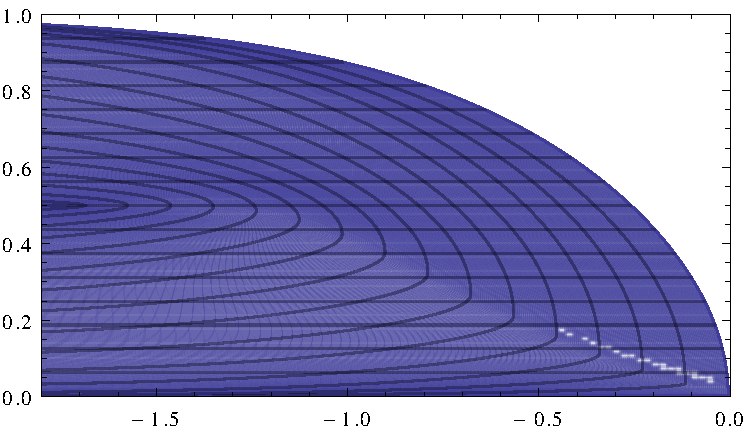
\includegraphics[scale=0.9]{remap_particle_paths.pdf}
\caption{Particle paths}
\label{}
\end{figure}

Note that $x_0$ varies from $0$ to $-1/\text{arctanh}(1/2)$ when $z_\infty$ goes from $0$ to $1/2$ (or from $1/2$ to $1$).
Therefore the pp "go back" to $x = -\infty$ only close to the head, in the finite region of space $[-1/\text{arctanh}(1/2);0]$.
I tend to think that the same thing happen with the velocity field of the flume paper, but this is only my feeling!

\section{Velocity field}

These pp seem rather similar to the one given by the velocity field used in the flume paper.
Now our job is to derive the velocity field corresponding to these new pp, and to inject it into our numerical solver to check if the desired spiralling structure will appear.

We have
\[
\frac{w}{u} = \frac{dz}{dx} = -\frac{(z_\infty - z_0)\left(1-\text{tanh}^2(-x+x_0)\right)}
		{2\sqrt{\text{tanh}(-x+x_0)}}
\]
Note that 
\[
\begin{matrix}
w  \xrightarrow[x \rightarrow -\infty]{} 0 \\
u  \xrightarrow[x \rightarrow x_0]{} 0
\end{matrix}
\]
as expected.
$w/u$ does not seem to depend on $z$, but recall that $z_\infty$ and $z_0$ are functions of $x_0 = x_0(x,z)$.
It is trivial to express $z$ as a function of $x$ and $x_0$, or $x$ as a function of $z$ and $x_0$:
\[
\begin{matrix}
z(x, x_0) = z_0(x_0) + (z_\infty(x_0) - z_0(x_0)) \sqrt {\text{tanh} (-x + x_0)} \\
x(z, x_0) = x_0 - \text{arctanh} \left[ \left( \frac{z - z_0(x_0)}{z_\infty(x_0) - z_0(x_0)} \right)^2 \right]
\end{matrix}
\]
However, expressing $x_0$ as an explicit function of $x$ and $z$ seem difficult.
Therefore it seems unlikely that we can have an explicit expression for $u$ and $w$ using these pp. However it is not hard to evaluate numerically $u$ and $w$. So what I would like to do if I had some time would be to do a numerical simulation using the numerically evaluated $u$ and $w$ to seem if we can observe the spiralling structure, as I believe we will. I would also like to try thinking of a simpler expression for the pp, a one simple enough to make it possible to have $u$ and $w$ explicitly. I believe it is not hard to find one. 

\section{Conclusion}

Despite of all of my efforts, I have not succeeded in describing analytically the structure of the steady-state solution for the flume problem in the 3D case. 
For now, I cannot tell if trying to do this remap is a good idea or not.
I think we should to take a closer look at the numerical solution.
I think we need to understand better how to describe this spiral we observe in terms of characteristics, shock waves and rarefaction waves.

I also think prescribing directly the particle paths could be a good idea. I am confident that in the end someone will describe this spiralling structure, because it seems universal. It always appear in the computations I ran, with very different velocity profiles. In my opinion it is sufficient to have $\partial v / \partial y \neq 0$ to observe this structure. I think that "forcing" the flow height to go to $0$ at $x=0$ is not required to observe it, though I have not tried not to do that.

What I would like to do next - if my internship was not over! It is a shame I had not the idea to look at this problem earlier, it really is an interesting one! - would be to try obtaining this spiral with the most simple setup: a constant flow height $H$, $w=v=0$, $ u ( x = 0 ) = - u ( x = H ) $ and $\partial v / \partial y \neq 0$ at some point in the flow, for example around $x = 0$.
Hopefully we will still have the spiral in that case, and it will be easier to understand what is going on!
\end{document}